\documentclass[tikz,border=4pt]{standalone}
\begin{document}
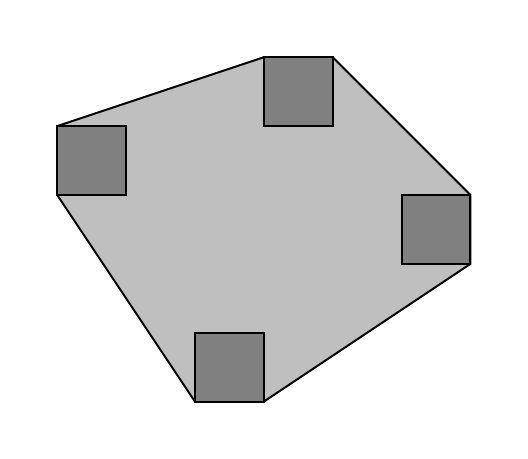
\begin{tikzpicture}[x=.025cm,y=-.025cm]
\path[use as bounding box] (0,0) rectangle (240,205);
\path[draw=black,fill=gray!50,line width=0.7150000000000001pt] (15,50) -- (120,15) -- (155,15) -- (225,85) -- (225,120) -- (120,190) -- (85,190) -- (15,85) -- cycle;
\path[draw=black,fill=gray,line width=0.7150000000000001pt] (15,50) -- (50,50) -- (50,85) -- (15,85) -- cycle;
\path[draw=black,fill=gray,line width=0.7150000000000001pt] (120,15) -- (155,15) -- (155,50) -- (120,50) -- cycle;
\path[draw=black,fill=gray,line width=0.7150000000000001pt] (190,85) -- (225,85) -- (225,120) -- (190,120) -- cycle;
\path[draw=black,fill=gray,line width=0.7150000000000001pt] (85,155) -- (120,155) -- (120,190) -- (85,190) -- cycle;
\end{tikzpicture}
\end{document}
